\chapter{Implementation}

\label{chap:impl}

\section{Design and Conception}

\label{sec:design_concept}

We are now focusing on the design and concept of the application. On an abstract level, the application should be a Representational State Transfer (REST) API with a database to store users, items and user ratings. This data should be available on the API along with recommendations and similarities.

\begin{figure}[h]
\centering
\includegraphics[width=\textwidth]{images/BPMN_design}
\caption{\label{fig:design}Application Concept}
\end{figure}

\subsection{Routing}

Below is a description of the API's web routes and how to interact with them.

For user data, there should be the following web routes:

\begin{longtable}{|p{2.5cm}|p{2.5cm}|p{3.2cm}|p{5cm}|}
    \hline
	  Name & Http Method & Route & Description \\
    \hline
    \hline
    User Info & GET & /user/<userid> & Returns the username and optional informations of the user \ref{code:user_info_json}\\
    \hline
    User Ratings & GET & /user/ratings & Should provide all ratings of all users \ref{code:user_ratings_json}\\
    \hline
    Create User & PUT & /user & Create a user, and takes a data object for name and in formations \ref{code:user_create_json}\\
    \hline
    Create User & DELETE & /user/<userid> & Dreate a user by it's userid\\
    \hline
    Add Rating & POST & /user/rating & Should create ratings defined in a data object \ref{code:user_reating_create_json}\\
    \hline
    All Users & GET & /users & Returns all users (id, name, information) \ref{code:user_infos_json}\\
    \hline
\end{longtable}

For the items we define the following web routes:

\begin{longtable}{|p{2.5cm}|p{2.5cm}|p{3.2cm}|p{5cm}|}
    \hline
	  Name & Http Method & Route & Description \\
    \hline
    \hline
    Item Info & GET & /item/<itemId> & Returns item name and description \ref{code:item_info_json}\\
    \hline
    Create Item & PUT & /item & Creates a item and takes the name and description form the provided data \ref{code:item_create_json}\\
    \hline
    Create Item & DELETE & /item/<itemId> & Deletes a item by it's item id\\
    \hline
    Modify Item & POST & /item & Updates the description and name of an item \ref{code:item_modify_json}\\
    \hline
    All Items & GET & /items & Returns all items (id, name, description) \ref{code:items_info_json}\\
    \hline
\end{longtable}

We also define the routes for the recommender system:

\begin{longtable}{|p{2.5cm}|p{2.5cm}|p{3.2cm}|p{5cm}|}
    \hline
	  Name & Http Method & Route & Description \\
    \hline
    \hline
    User Similarities & GET & /userBased/\allowbreak similarities/\allowbreak<userid> & Returns all user similarities for the specified user \ref{code:user_sim_json}\\
    \hline
    Userbased Recommendations & GET & /userBased/\allowbreak recommendations/\allowbreak<userid> & Returns all unrated items for the specified user with an estimated rating\\
    \hline
    Items Similarities & GET & /userBased/\allowbreak similarities/\allowbreak<itemId> & Returns all item similarities for the specified item\\
    \hline
    Itembased Recommendations & GET & /userBased/\allowbreak recommendations/\allowbreak <itemId> & Returns all unrated items for the specified user with an estimated rating\\
    \hline
\end{longtable}

\subsection{Recommender}

We will now look at the design of the recommender system. We divide the recommender system into components: 

\begin{itemize}
    \item A controller that retrieves data and puts it into the necessary components
    \item The similarity measure, which allows the recommender system to compare two users or items
    \item selection algorithms to select only the most relevant items and users to make a recommendation
\end{itemize}

The interactions and relationships between the components are shown in \ref{fig:recommender_design}.
\newpage

\begin{figure}[h]
\centering
\includegraphics[width=\textwidth]{images/BPM_recommender_design}
\caption{\label{fig:recommender_design}description}
\end{figure}


\section{Technologies}

\label{sec:technologies}

\subsection{Kotlin Framework Ktor}

Ktor is a web framework for building web services, clients or applications that connect over the web. Ktor uses coroutines to achieve an asynchronous context to provide an efficient framework for developers.

In this paper we will mainly use the Ktor server dependencies, and only use the Ktor client if the application needs to make requests to other services.

\subsection{Kotlin Library Ktorm}

Ktorm is a database Object Relational Mapping (ORM) for Structured Query Language (SQL) databases written in Kotlin. It provides a strongly typed SQL DSL for constructing SQL queries \cite{Ktorm}. A DSL or type-safe builder \cite{DSL} can help provide a builder that is statically typed and type-safe. This forces a developer to write correct SQL statements.

Ktorm also handles the connection to the database and keeps the tables as Kotlin objects for easy interaction with the database.

\subsection{Ktor Plugins}

Additional dependencies we use are available as Ktor plugins, this way the Ktor framework handles the initialisation of these dependencies and provides them when needed.

\subsubsection{Koin}

Koin is a dependency injection framework that is available for the Kotlin programming language \cite{Koin}. In this Application we use Koin to manage Objects like a Database object that is shared between asynchronous Routes and make it accessible.

We start Koin at the start of the application within Ktor:

\begin{minted}[frame=lines,framesep=2mm,baselinestretch=1.2,fontsize=\footnotesize,bgcolor=LightGray]{kotlin}
fun Application.configureKoin(vararg appModules: Module) {
    install(Koin) {
        slf4jLogger()
        modules(appModules.toList())
    }
}
\end{minted}

We define the application module in the defined entry point of Ktor:

\newpage

\begin{minted}[frame=lines,framesep=2mm,baselinestretch=1.2,fontsize=\footnotesize,bgcolor=LightGray]{kotlin}
    val config = ConfigLoader().loadConfig().getOrElse { it ->
        log.error(it.message)
        this.dispose()
        return
    }
    val logger = LoggerFactory.getLogger("api")

    val appModules = org.koin.dsl.module {
        single { config }
        single(qualifier("main")) { config.databases.main }
        single { logger }
        single { BpmDatabase() }
        single { JwtConfig(config.token) }
    }
\end{minted}


\subsubsection{CORS}

The application also defines CORS or Cross-Origin Resource Sharing. This is where a web application references another web application in the browser, rather than calling the application itself. This causes the browser to access a different URL from within the website, which is restricted by most browsers as it prevents potentially malicious third-party scripts from being executed. The author of this paper strongly discourages this approach, as the API was not designed to be accessed from a browser. We recommend that requests to this API are made from a server that handles user authentication.

When deploying the application, allowed hosts can be defined in the config.yaml \ref{code:App_conf_yml}.

\subsubsection{Authentication}

For a client to access the different routes on the API, Json Web Tokens or JWT are used for authentication. To configure this feature we install the authentication plugin with the JWT extension.

\begin{minted}[frame=lines,framesep=2mm,baselinestretch=1.2,fontsize=\footnotesize,bgcolor=LightGray]{kotlin}
fun Application.configureSecurity(jwtConfig: JwtConfig) {
    authentication {
        jwt {
            jwtConfig.configureKtorFeature(this)
        }
    }
}
\end{minted}

In this case more configuration is needed as we can save some data within the JWT and access this data within a request. The JWT configuration can be found in \ref{code:JWT_conf}. An authenticated route using JWT might look like this:

\begin{minted}[frame=lines,framesep=2mm,baselinestretch=1.2,fontsize=\footnotesize,bgcolor=LightGray]{kotlin}
fun Application.authenticatedRoute() {
    routing {
        authenticate {
            get("/route") {
                val principal = call.principal<JwtConfig.User>()
                application.log.debug(principal?.userinfo)
            }
        }
    }
}
\end{minted}

\subsubsection{Serialization}

The application uses JSON as Content Negotiation as defined in the functional requirements. The kotlin serialization plugin in combination with Ktorm enables the Application to send Kotlin Objects while the serialization plugin transform the objects to JSON and also transforms JSON within a http body to Kotlin object. 

\begin{minted}[frame=lines,framesep=2mm,baselinestretch=1.2,fontsize=\footnotesize,bgcolor=LightGray]{kotlin}
fun Application.configureSerialization() {
    install(ContentNegotiation) {
        json()
    }
}
\end{minted}

\section{Architecture}

\label{sec:architecture}

In this section we will describe the implementation of the software discussed in the design phase \ref{sec:design_concept}. We also define other necessary components that are relevant, such as dependencies or the server framework. 

\subsection{Application Startup}

The entry point of the application is a NettyApplicationEngine provided by Ktor, we make a change so that when the application is started, command line arguments can be passed to the engine.

\begin{minted}[frame=lines,framesep=2mm,baselinestretch=1.2,fontsize=\footnotesize,bgcolor=LightGray]{kotlin}
fun main(args: Array<String>) {
    val applicationEnvironment = commandLineEnvironment(args)
    NettyApplicationEngine(applicationEnvironment) {
        loadConfiguration(applicationEnvironment.config)
    }.start(true)
}
\end{minted}

After starting the engine, Ktor will look for an application.conf \ref{code:ktor_app_conf} defined in the resource directory and look for an entry point. The entry point implementation can be found in \ref{code:app_entry_point}.

We also load a configuration \ref{code:App_conf_loading} for database access and a secret token to create JWT tokens.

To get a better overview of the whole start-up process, see diagram \ref{fig:startup}.

\begin{figure}[h!]
\centering
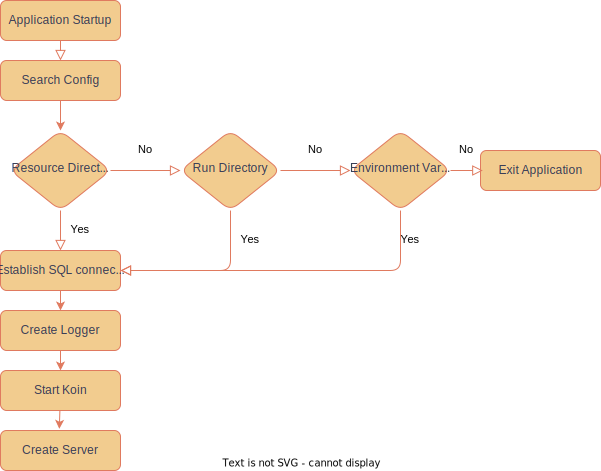
\includegraphics[width=\textwidth]{images/StartupBachelor.drawio.png}
\caption{\label{fig:startup}Application startup}
\end{figure}

\newpage

\subsection{Routing}

As indicated in the design and concept section, we divided web routes into three classes to handle user, item and recommendation requests. After the startup procedure described in \ref{fig:startup}, we can initialise the three classes and inject the necessary data using Koin also shown in figure \ref{fig:routing}.

\begin{figure}[h!]
\centering
\includegraphics[width=\textwidth]{images/RoutingUML.png}
\caption{\label{fig:routing}Routing UML class diagram}
\end{figure}

\newpage

Within these routes, we authenticate the request:

\begin{minted}[frame=lines,framesep=2mm,baselinestretch=1.2,fontsize=\footnotesize,bgcolor=LightGray]{kotlin}
suspend fun PipelineContext<Unit, ApplicationCall>.bpmnAuth(
    routeInfo: String,
    logger: Logger,
): Boolean {
    val principal = call.principal<JwtConfig.User>()
    val hasAccess: Boolean = (principal?.role == "admin")
    val noToken: Boolean = principal == null

    val success = "Successfully authenticated " +
        "'${principal?.userinfo}' to access '$routeInfo'!"
    val denied = "Denied access for '$principal' to access " +
        "'$routeInfo'!"

    val unAuthMsg = "Please reauthenticate!"
    val forbidden =
        "You don't have the correct role to access " +
            "this Route!"

    return if (hasAccess) {
        logger.info(success)
        true
    } else if (noToken) {
        logger.warn(denied)
        call.respond(HttpStatusCode.Unauthorized, unAuthMsg)
        false
    } else {
        logger.warn(denied)
        call.respond(HttpStatusCode.Forbidden, forbidden)
        false
    }
}
\end{minted}

In a route, for example, when you try to change an item's information, it will look like this:

\begin{minted}[frame=lines,framesep=2mm,baselinestretch=1.2,fontsize=\footnotesize,bgcolor=LightGray]{kotlin}
private fun Route.modifyItem() {
    post {
        val authenticated = bpmnAuth(
            routeInfo = "/items/",
            logger
        )
        if (!authenticated) {
            return@post
        }
        val data = call.receive<Item>()

        val effectedRows = database.itemDao.modifyItem(
            data
        )
        if (effectedRows == 1) {
            call.respond(HttpStatusCode.OK)
        } else {
            call.respond(
                HttpStatusCode.InternalServerError,
                "Something went wrong: $effectedRows effected rows!"
            )
        }
    }
}
\end{minted}

\subsection{Database Access Objects}

To access the database with ktorm, we introduce a database access object (DAO). We modify the dataflow described in the design section and introduce a DAO that contains all the queries we need, as seen in figure \ref{fig:dao_vis}.

\begin{figure}[h!]
\centering
\includegraphics[width=\textwidth]{images/dao_visualizer.png}
\caption{\label{fig:dao_vis}Database Access Object}
\end{figure}

\newpage

Within the DAO, we now define queries using the Ktrom ORM DSL, for example to get all users:

\begin{minted}[frame=lines,framesep=2mm,baselinestretch=1.2,fontsize=\footnotesize,bgcolor=LightGray]{kotlin}
fun getAllUsers(): EntitySequence<UserDbEntity, UserDbTable> {
    return database.sequenceOf(UserDbTable)
}
\end{minted}

While the user table in Kotlin is defined like this:

\begin{minted}[frame=lines,framesep=2mm,baselinestretch=1.2,fontsize=\footnotesize,bgcolor=LightGray]{kotlin}
interface UserDbEntity : Entity<UserDbEntity> {
    companion object : Entity.Factory<UserDbEntity>()
    val id: Int
    val name: String
    val info: String?
}
object UserDbTable : Table<UserDbEntity>("bpm_user") {
    val id = int("id").primaryKey().bindTo { it.id }
    val name = varchar("name").bindTo { it.name }
    val info = text("info").bindTo { it.info }
}
\end{minted}

\section{Recommendation Algorithms}

\label{sec:recommend_algo}

\subsection{Similarity Measures}

All similarity measures implement an interface to facilitate the use of the algorithms.

\begin{minted}[frame=lines,framesep=2mm,baselinestretch=1.2,fontsize=\footnotesize,bgcolor=LightGray]{kotlin}
interface SimilarityMeasure {
    /**
     * compares 2 data maps and returns a similarity measure,
     * note: comparing the result of this function only works 
     * with the same Similarity Measure!
     *
     * @param dataA the first data set
     * (key: the item, value: the rating of the item)
     * @param dataB the second data set
     * (key: the item, value: the rating of the item)
     * @param allItems all the items referenced in data1 & 2
     */
    fun compare(
        dataA: Map<String, Int>,
        dataB: Map<String, Int>,
        allItems: List<String>
    ): Number
}
\end{minted}

This way, similarity measures are easily extensible.

\subsubsection{Euclid}

The Euclidean algorithm can calculate similarity based on distance. In other words, if the distance between two users is small, they are more similar. The dimension n is the number of items.

\begin{equation}
S_{e} = \frac{1}{1+\sqrt{\sum_{i=1}^{n}{(dataA_i - dataB_i)^2}}}
\label{euklid}
\end{equation}

DataA and DataB refer to the ratings of two different users or items.
The implementation in Kotlin is as follows:

\begin{minted}[frame=lines,framesep=2mm,baselinestretch=1.2,fontsize=\footnotesize,bgcolor=LightGray]{kotlin}
class Euclid : SimilarityMeasure {
    override fun compare(
        dataA: Map<String, Int>,
        dataB: Map<String, Int>,
        allItems: List<String>,
    ): Number {
        val sum = allItems.sumOf {
            ((dataA[it] ?: 0) - (dataB[it] ?: 0))
                .toDouble().pow(2)
        }

        return 1 / (1 + sqrt(sum))
    }
}
\end{minted}

The difference of the ratings of DataA and DataB is an integer, but is converted to a double because the pow() function in the Kotlin standard library is only defined for floats and doubles.

\subsubsection{Cosine}

The basic calculation is separated into the companion object of the class as the calculation is also used by the Pearson distance measure. The cosine measure can be calculated as follows:

\begin{equation}
S_{c} = \frac{\sum_{i=1}^{n}{dataA_i * dataB_i}}{\sqrt{\sum_{i=1}^{n}{(dataA_i)^2} * \sum_{i=1}^{n}{(dataB_i)^2}}}
\label{eq:cosine}
\end{equation}

The implementation in Kotlin looks like this:

\newpage

\begin{minted}[frame=lines,framesep=2mm,baselinestretch=1.2,fontsize=\footnotesize,bgcolor=LightGray]{kotlin}
class Cosine : SimilarityMeasure {
    companion object {
        fun basicCalc(
            dataA: Map<String, Number>,
            dataB: Map<String, Number>,
            allItems: List<String>,
        ): Number {
            var sumATimesB = 0.0
            var sumASquared = 0.0
            var sumBSquared = 0.0

            allItems.forEach {
                sumATimesB += (dataA[it] ?: 0).toDouble() * 
                    (dataB[it] ?: 0).toDouble()
                sumASquared += (dataA[it] ?: 0).toDouble().pow(2)
                sumBSquared += (dataB[it] ?: 0).toDouble().pow(2)
            }

            return (sumATimesB / (sqrt(sumASquared * sumBSquared)))
        }
    }

    override fun compare(
        dataA: Map<String, Int>,
        dataB: Map<String, Int>,
        allItems: List<String>,
    ): Number {
        return basicCalc(dataA, dataB, allItems)
    }
}
\end{minted}

\subsubsection{Pearson}

The Pearson distance measure now calculates the correlation coefficient and uses the cosine measure with the modified data to get it's distance. To get the correlation coefficient, we add up all of a user's ratings and divide by the number of ratings.

\begin{minted}[frame=lines,framesep=2mm,baselinestretch=1.2,fontsize=\footnotesize,bgcolor=LightGray]{kotlin}
object CorrelationCoefficient {
    /**
     * calculates the Correlation Coefficient for one person
     * and their recommendations
     *
     * @param list the items a user has rated
     */
    fun calculate(list: List<Int>): Float {
        return list.sum() / list.size.toFloat()
    }
}
\end{minted}

We can now subtract the correlation coefficient on each item rating and use the cosine distance measure to calculate.

\begin{minted}[frame=lines,framesep=2mm,baselinestretch=1.2,fontsize=\footnotesize,bgcolor=LightGray]{kotlin}
class Pearson : SimilarityMeasure {
    override fun compare(
        dataA: Map<String, Int>,
        dataB: Map<String, Int>,
        allItems: List<String>,
    ): Number {
        val correlationCoefficientA =
            CorrelationCoefficient
                .calculate(dataA.values.toList())
        val correlationCoefficientB =
            CorrelationCoefficient
                .calculate(dataB.values.toList())
        return (Cosine.basicCalc(
                dataA.mapValues { (_, value) ->
                    value - correlationCoefficientA
                },
                dataB.mapValues { (_, value) ->
                    value - correlationCoefficientB
                }.toMap(),
                allItems
            ).toDouble() + 1) / 2
    }
}
\end{minted}

At the end of Pearson we add one and divide by two. We do this because pearson can produce similarities between negative one and one. To calculate a weighted average recommendation, we need the similarities to be between zero and one.

\subsection{Knn}

Getting the k nearest neighbours is straightforward after getting the similarities. We select users or items based on the highest similarity.

\begin{minted}[frame=lines,framesep=2mm,baselinestretch=1.2,fontsize=\footnotesize,bgcolor=LightGray]{kotlin}
object Knn {
    /**
     * calculate the k nearest neighbours
     *
     * @param neighbors all the neighbours that the [Recommender] 
     * has calculated
     * @param k select the k nearest
     * @return the k nearest neighbours
     */
    fun calculate(
        neighbors: List<Recommender.UserSimilarity>,
        k: Int,
    ): List<Recommender.UserSimilarity> {
        return neighbors.sortedBy { it.similarity }.takeLast(k)
    }
}
\end{minted}

\subsection{Average}

Having found the k nearest neighbours, we can now take the average or weighted average of the ratings of the neighbours found.

\newpage

\begin{minted}[frame=lines,framesep=2mm,baselinestretch=1.2,fontsize=\footnotesize,bgcolor=LightGray]{kotlin}
object Mean {
    fun weightedMean(
        userSimilarity: List<Recommender.UserSimilarity>,
        item: String,
    ): Double {
        return userSimilarity.sumOf {
            it.ratings[item]!! * it.similarity
        } / userSimilarity.sumOf { it.similarity }
    }

    fun mean(
        userSimilarity: List<Recommender.UserSimilarity>,
        item: String,
    ): Double {
        return userSimilarity.sumOf {
            it.ratings[item]!!
        }.toDouble() / userSimilarity.size
    }
}
\end{minted}

\section{Development Process}

\label{sec:dev_process}

We will now briefly discuss the development process, the tools used and the problems encountered during development.

\subsection{Tools}

During development, several tools were used to make the development process easier and more efficient.

\begin{itemize}
    \item Github was used for version control and to make the software accessible. Github was also used to plan and document the software through Github projects, where a roadmap and overview of all issues were created
    \item Docker Desktop was used to manage Docker containers and images.
    \item Intelij IDEA was used as the primary development environment, which also managed the connection to github and sql during development.
\end{itemize}

\subsection{Problems during the Development}

There are some issues that came up during development and we want to discuss them. Within these problems, there were no major issues that needed to be resolved.

\begin{itemize}
    \item When calculating similarities between items or users, there is the possibility of a division by zero, which is a problem because within JSON, the NaN value provided by the serialisation plugin for Kotlin is not valid for numbers and violates JSON conventions.
    \item The Gradle project and the API source code were initially in a separate folder within the project, which was a problem for Intelij as it wasn't possible to import, build and run the Gradle project.
    \item The gradlew file was missing the execution flags to run within a Github Action, this was a problem as there is no easy way on Windows to change the Linux based file flags.
    \item Some similarity measures produce negative similarities, which is a problem because the recommendations should not be negative when calculating the weighted average of the ratings.
\end{itemize}
